\section{Partial Derivatives}
\label{sec:partial-derivatives}

Most physical systems depend on several independent variables. A temperature field may vary with three spatial coordinates and time, a thermodynamic state function may depend on pressure and volume, and a quantum wavefunction may depend on position, spin coordinates, and time. Partial differentiation extends the derivative to such multivariable functions by isolating the response to one variable while the remaining independent variables are held fixed.

The central idea is local. Near a point, a sufficiently smooth multivariable function is approximated by a plane or, in higher dimensions, by a linear map. Its partial derivatives are the coefficients of this approximation. They therefore provide the raw material for gradients, Jacobians, Hessians, differential equations, and the field theories used throughout physics.

\begin{bookhistory}[From Curves to Fields]
Ordinary differential calculus was developed for functions of one variable, but mechanics, thermodynamics, and field theory quickly required functions of several variables. Euler, Lagrange, Laplace, Fourier, and later Gibbs and Maxwell transformed partial differentiation into a basic language of mathematical physics. Modern quantum mechanics continues this tradition: the Schr\"odinger equation is a partial differential equation because the wavefunction depends simultaneously on space and time.
\end{bookhistory}

\subsection{Functions of Several Variables}

A scalar-valued function of two variables has the form

\[
f:\mathbb{R}^2\rightarrow\mathbb{R},
\qquad
(x,y)\mapsto f(x,y).
\]

Its graph is the surface

\[
z=f(x,y)
\]

in three-dimensional space. A function of three spatial coordinates,

\[
\phi(x,y,z),
\]

is more naturally interpreted as a scalar field: each point of space is assigned a number such as temperature, pressure, density, or electric potential.

\begin{bookexample}[Temperature Field]
Suppose
\[
T(x,y,z)=T_0-\alpha(x^2+y^2)-\beta z,
\]
where $T_0$, $\alpha$, and $\beta$ are constants. The temperature changes differently in different directions. Moving in the $x$-direction produces a change governed by $-2\alpha x$, moving in the $y$-direction produces $-2\alpha y$, and moving vertically produces the constant change $-\beta$.
\end{bookexample}

\subsection{Rigorous Definition from a Limit}

Fix a point $(a,b)$ in the domain of $f(x,y)$. To study change in the $x$-direction, hold $y=b$ fixed and vary only $x$. The resulting one-variable slice is

\[
g(x)=f(x,b).
\]

The ordinary derivative of this slice at $x=a$ defines the partial derivative with respect to $x$.

\begin{bookdefinition}[Partial Derivative with Respect to $x$]
The partial derivative of $f$ with respect to $x$ at $(a,b)$ is
\begin{equation}
\boxed{
\frac{\partial f}{\partial x}(a,b)
=
\lim_{h\to0}
\frac{f(a+h,b)-f(a,b)}{h}
}
\label{eq:partial-x-limit}
\end{equation}
provided the limit exists and is finite.
\end{bookdefinition}

Similarly,

\begin{equation}
\boxed{
\frac{\partial f}{\partial y}(a,b)
=
\lim_{k\to0}
\frac{f(a,b+k)-f(a,b)}{k}
}
\label{eq:partial-y-limit}
\end{equation}

holds $x=a$ fixed and varies only $y$.

Common notations include

\[
f_x,
\qquad
\partial_x f,
\qquad
\frac{\partial f}{\partial x},
\qquad
D_xf.
\]

\begin{bookremark}[What ``Holding the Other Variables Fixed'' Means]
The phrase does not mean that the other quantities can never change physically. It means that the mathematical experiment defining one partial derivative compares nearby points that differ in only one coordinate. Other changes are included later through the total differential or total derivative.
\end{bookremark}

\subsection{Partial Derivatives from First Principles}

Consider

\[
f(x,y)=x^2y+3y^2.
\]

Using the limit definition,

\begin{align*}
\frac{\partial f}{\partial x}(x,y)
&=
\lim_{h\to0}
\frac{f(x+h,y)-f(x,y)}{h}\\
&=
\lim_{h\to0}
\frac{(x+h)^2y+3y^2-(x^2y+3y^2)}{h}\\
&=
\lim_{h\to0}
\frac{2xyh+yh^2}{h}\\
&=
\lim_{h\to0}(2xy+yh)\\
&=2xy.
\end{align*}

Likewise,

\begin{align*}
\frac{\partial f}{\partial y}(x,y)
&=
\lim_{k\to0}
\frac{x^2(y+k)+3(y+k)^2-(x^2y+3y^2)}{k}\\
&=
\lim_{k\to0}
\left(x^2+6y+3k\right)\\
&=x^2+6y.
\end{align*}

Therefore

\[
\boxed{
f_x=2xy,
\qquad
f_y=x^2+6y.
}
\]

\begin{bookexample}[Exponential and Trigonometric Dependence]
Let
\[
f(x,y)=e^{xy}\sin(x+y).
\]
Treating $y$ as constant,
\[
f_x
=
ye^{xy}\sin(x+y)+e^{xy}\cos(x+y).
\]
Treating $x$ as constant,
\[
f_y
=
xe^{xy}\sin(x+y)+e^{xy}\cos(x+y).
\]
The expressions differ because the product $xy$ responds differently to changes in $x$ and $y$.
\end{bookexample}

\begin{bookexample}[Three Variables]
For
\[
f(x,y,z)=x^2e^{yz}+z\cos x,
\]
one obtains
\[
f_x=2xe^{yz}-z\sin x,
\]
\[
f_y=x^2ze^{yz},
\]
and
\[
f_z=x^2ye^{yz}+\cos x.
\]
\end{bookexample}

\subsection{Geometric Interpretation}

For the surface $z=f(x,y)$, fixing $y=b$ produces the curve

\[
z=f(x,b).
\]

The number $f_x(a,b)$ is the slope of the tangent line to this curve at $(a,b,f(a,b))$. Fixing $x=a$ gives a second coordinate curve whose tangent slope is $f_y(a,b)$.

\begin{figure}[htbp]
\centering
\begin{tikzpicture}[scale=0.95]
\draw[->] (-0.3,0) -- (6.2,0) node[right] {$x$};
\draw[->] (0,-0.3) -- (0,4.8) node[above] {$z$};
\draw[domain=0.3:5.7,smooth,variable=\x,thick] plot ({\x},{0.13*(\x-3)^2+1.0});
\coordinate (P) at (3,1);
\fill (P) circle (2.2pt) node[below right] {$P$};
\draw[thick,dashed] (1.1,1.0) -- (5.2,1.0) node[right] {tangent for fixed $y$};
\node at (3.6,3.6) {$z=f(x,b)$};
\end{tikzpicture}
\caption{A partial derivative is an ordinary derivative along a coordinate slice of the surface.}
\label{fig:partial-coordinate-slice}
\end{figure}

The two partial derivatives describe slopes along the coordinate directions, but a surface has infinitely many possible directions. Directional derivatives will combine these coordinate slopes into a general directional rate of change.

\subsection{Continuity, Partial Derivatives, and Differentiability}

The existence of $f_x$ and $f_y$ at a point does not by itself guarantee that $f$ is continuous or differentiable there. Multivariable differentiability is stronger: the function must admit one linear approximation that works for all sufficiently small directions simultaneously.

\begin{bookdefinition}[Differentiability in Two Variables]
A function $f$ is differentiable at $(a,b)$ if there exists a linear expression
\[
L(h,k)=Ah+Bk
\]
such that
\begin{equation}
f(a+h,b+k)
=
f(a,b)+Ah+Bk+r(h,k),
\label{eq:multivariable-differentiability}
\end{equation}
where
\[
\lim_{(h,k)\to(0,0)}
\frac{r(h,k)}{\sqrt{h^2+k^2}}=0.
\]
In that case $A=f_x(a,b)$ and $B=f_y(a,b)$.
\end{bookdefinition}

A standard sufficient condition is especially useful.

\begin{bookproperty}[Continuous Partials Imply Differentiability]
If $f_x$ and $f_y$ exist in a neighbourhood of $(a,b)$ and are continuous at $(a,b)$, then $f$ is differentiable at $(a,b)$.
\end{bookproperty}

\begin{bookwarning}[Existing Partials Are Not Enough]
It is possible for both coordinate partial derivatives to exist at a point while the function behaves badly along diagonal or curved paths. Differentiability requires control in every direction, not only along the coordinate axes.
\end{bookwarning}

\subsection{Tangent Plane and Linear Approximation}

For a differentiable surface $z=f(x,y)$ near $(a,b)$, Eq.~\eqref{eq:multivariable-differentiability} gives

\[
f(a+h,b+k)
\approx
f(a,b)+f_x(a,b)h+f_y(a,b)k.
\]

Since $h=x-a$ and $k=y-b$, the tangent plane is

\begin{equation}
\boxed{
z
=
f(a,b)
+f_x(a,b)(x-a)
+f_y(a,b)(y-b).
}
\label{eq:tangent-plane}
\end{equation}

\begin{bookprinciple}[Best Local Plane]
The tangent plane is not merely a plane touching the surface. It is the unique affine function whose error becomes negligible compared with the distance from $(a,b)$ as the point approaches $(a,b)$.
\end{bookprinciple}

\begin{bookexample}[Tangent Plane]
Let
\[
f(x,y)=x^2+xy+y^2.
\]
At $(1,2)$,
\[
f(1,2)=7,
\qquad
f_x=2x+y,
\qquad
f_y=x+2y,
\]
so
\[
f_x(1,2)=4,
\qquad
f_y(1,2)=5.
\]
The tangent plane is therefore
\[
\boxed{
z=7+4(x-1)+5(y-2).}
\]
At $(1.02,1.97)$, the linear estimate gives
\[
z\approx7+4(0.02)+5(-0.03)=6.93.
\]
\end{bookexample}

\begin{figure}[htbp]
\centering
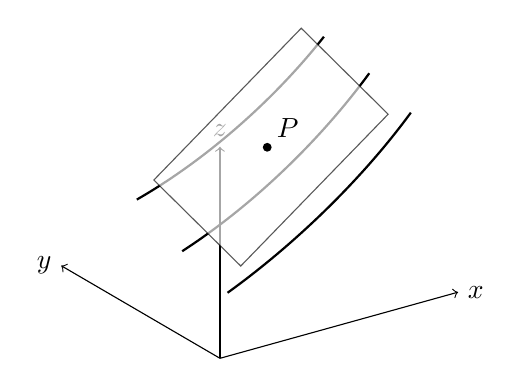
\begin{tikzpicture}[x={(0.9cm,0.25cm)},y={(-0.6cm,0.35cm)},z={(0cm,0.8cm)},scale=0.8]
\draw[->] (0,0,0)--(4.2,0,0) node[right]{$x$};
\draw[->] (0,0,0)--(0,4.2,0) node[left]{$y$};
\draw[->] (0,0,0)--(0,0,4.2) node[above]{$z$};
\draw[thick] (0.4,0.4,1.0) .. controls (1.6,0.5,1.5) and (2.8,0.5,2.4) .. (3.7,0.5,3.5);
\draw[thick] (0.4,1.6,1.3) .. controls (1.6,1.6,1.8) and (2.8,1.6,2.7) .. (3.7,1.6,3.8);
\draw[thick] (0.4,2.8,1.8) .. controls (1.6,2.8,2.2) and (2.8,2.8,3.0) .. (3.7,2.8,4.0);
\filldraw[fill=white,opacity=0.65] (0.9,0.8,1.2)--(3.5,0.8,3.4)--(3.5,3.1,4.1)--(0.9,3.1,1.9)--cycle;
\fill (2.1,1.9,2.7) circle (2pt) node[above right]{$P$};
\end{tikzpicture}
\caption{A differentiable surface is locally approximated by its tangent plane.}
\label{fig:tangent-plane-surface}
\end{figure}

\subsection{Total Differential}

For a differentiable function $f(x,y)$, the first-order change is

\begin{equation}
\boxed{
df
=
f_x\,dx+f_y\,dy.
}
\label{eq:total-differential-2d}
\end{equation}

For $f(x,y,z)$,

\begin{equation}
\boxed{
df
=
f_x\,dx+f_y\,dy+f_z\,dz.
}
\label{eq:total-differential-3d}
\end{equation}

This follows directly from the linear approximation. If $\Delta x$, $\Delta y$ are small, then

\[
\Delta f
=
f_x\Delta x+f_y\Delta y+	ext{higher-order error},
\]

and the total differential retains the first-order part.

\begin{bookexample}[Propagation of Measurement Uncertainty]
For the area of a rectangle,
\[
A(L,W)=LW,
\]
the differential is
\[
dA=W\,dL+L\,dW.
\]
If $L=2.00\,\mathrm{m}$, $W=1.50\,\mathrm{m}$, $|dL|=0.01\,\mathrm{m}$, and $|dW|=0.02\,\mathrm{m}$, then a conservative first-order estimate is
\[
|dA|
\leq
W|dL|+L|dW|
=1.50(0.01)+2.00(0.02)
=0.055\,\mathrm{m}^2.
\]
\end{bookexample}

\subsection{Total Derivative and the Multivariable Chain Rule}

If $x=x(t)$ and $y=y(t)$, then

\begin{equation}
\boxed{
\frac{df}{dt}
=
\frac{\partial f}{\partial x}\frac{dx}{dt}
+
\frac{\partial f}{\partial y}\frac{dy}{dt}.
}
\label{eq:total-derivative-two-vars}
\end{equation}

For $f(x,y,z,t)$ evaluated along a moving trajectory $\mathbf r(t)$,

\begin{equation}
\boxed{
\frac{df}{dt}
=
\frac{\partial f}{\partial t}
+
\frac{\partial f}{\partial x}\dot x
+
\frac{\partial f}{\partial y}\dot y
+
\frac{\partial f}{\partial z}\dot z.
}
\label{eq:material-chain-rule}
\end{equation}

This distinction is fundamental in physics: $\partial f/\partial t$ measures local time change at a fixed point, whereas $df/dt$ measures the change experienced by an observer moving through the field.

\begin{bookexample}[Temperature Experienced by a Moving Probe]
Let
\[
T(x,y,t)=100-2x^2-y^2+3t,
\]
and let a probe move along
\[
x=t,
\qquad
y=2t.
\]
Then
\[
T_t=3,
\qquad
T_x=-4x,
\qquad
T_y=-2y,
\]
so
\[
\frac{dT}{dt}=3-4x\dot x-2y\dot y.
\]
Since $\dot x=1$, $\dot y=2$, $x=t$, and $y=2t$,
\[
\boxed{\frac{dT}{dt}=3-12t.}
\]
\end{bookexample}

\subsection{Directional Derivatives}

Let $\mathbf u=(u_x,u_y)$ be a unit vector. The directional derivative of $f$ at $\mathbf a=(a,b)$ in the direction $\mathbf u$ is

\begin{equation}
\boxed{
D_{\mathbf u}f(\mathbf a)
=
\lim_{h\to0}
\frac{f(\mathbf a+h\mathbf u)-f(\mathbf a)}{h}.
}
\label{eq:directional-derivative-limit}
\end{equation}

For a differentiable function,

\begin{equation}
\boxed{
D_{\mathbf u}f
=
f_xu_x+f_yu_y
=
\nabla f\cdot\mathbf u.
}
\label{eq:directional-gradient}
\end{equation}

Although the gradient is developed fully in the next section, Eq.~\eqref{eq:directional-gradient} already shows why partial derivatives are its components.

\begin{bookexample}[Directional Rate of Change]
Let
\[
f(x,y)=x^2+3xy.
\]
At $(1,2)$,
\[
f_x=2x+3y=8,
\qquad
f_y=3x=3.
\]
For the unit direction
\[
\mathbf u=\frac{1}{5}(3,4),
\]
we find
\[
D_{\mathbf u}f
=8\frac35+3\frac45
=\frac{36}{5}.
\]
\end{bookexample}

\subsection{Second and Mixed Partial Derivatives}

Repeated differentiation produces

\[
f_{xx}=\frac{\partial^2f}{\partial x^2},
\qquad
f_{yy}=\frac{\partial^2f}{\partial y^2},
\]

and the mixed derivatives

\[
f_{xy}=\frac{\partial}{\partial y}\left(\frac{\partial f}{\partial x}\right),
\qquad
f_{yx}=\frac{\partial}{\partial x}\left(\frac{\partial f}{\partial y}\right).
\]

\begin{bookproperty}[Clairaut--Schwarz Theorem]
If the mixed second partial derivatives are continuous in a neighbourhood of a point, then
\[
\boxed{f_{xy}=f_{yx}.}
\]
\end{bookproperty}

\begin{bookexample}[Mixed Partials]
For
\[
f(x,y)=x^3y^2+e^{xy},
\]
one has
\[
f_x=3x^2y^2+ye^{xy},
\]
so
\[
f_{xy}=6x^2y+e^{xy}+xye^{xy}.
\]
Starting from
\[
f_y=2x^3y+xe^{xy}
\]
gives the same result for $f_{yx}$.
\end{bookexample}

\subsection{The Jacobian Matrix}

For a vector-valued function

\[
\mathbf F:\mathbb R^n\to\mathbb R^m,
\qquad
\mathbf F=(F_1,\ldots,F_m),
\]

the first-order partial derivatives form the Jacobian matrix

\begin{equation}
\boxed{
J_{\mathbf F}
=
\begin{pmatrix}
\dfrac{\partial F_1}{\partial x_1} & \cdots & \dfrac{\partial F_1}{\partial x_n}\\[6pt]
\vdots & \ddots & \vdots\\[6pt]
\dfrac{\partial F_m}{\partial x_1} & \cdots & \dfrac{\partial F_m}{\partial x_n}
\end{pmatrix}.
}
\label{eq:jacobian-matrix}
\end{equation}

The Jacobian is the best local linear map associated with $\mathbf F$. If $m=n$, its determinant measures the local signed change of volume.

\begin{bookexample}[Planar Mapping]
Let
\[
u=x^2-y^2,
\qquad
v=2xy.
\]
Then
\[
J
=
\begin{pmatrix}
2x & -2y\\
2y & 2x
\end{pmatrix},
\qquad
\det J=4(x^2+y^2).
\]
Away from the origin, the map locally expands area by the factor $4(x^2+y^2)$.
\end{bookexample}

\subsection{Jacobian Determinants and Coordinate Transformations}

For polar coordinates,

\[
x=r\cos\theta,
\qquad
y=r\sin\theta,
\]

the Jacobian is

\[
\frac{\partial(x,y)}{\partial(r,\theta)}
=
\begin{vmatrix}
\cos\theta & -r\sin\theta\\
\sin\theta & r\cos\theta
\end{vmatrix}
=r.
\]

Thus the area element transforms as

\begin{equation}
\boxed{dx\,dy=r\,dr\,d\theta.}
\label{eq:polar-area-element}
\end{equation}

For cylindrical coordinates,

\[
dV=r\,dr\,d\theta\,dz,
\]

and for spherical coordinates,

\begin{equation}
\boxed{
dV=r^2\sin\theta\,dr\,d\theta\,d\phi.
}
\label{eq:spherical-volume-element}
\end{equation}

The factors $r$ and $r^2\sin\theta$ are not arbitrary conventions. They are Jacobian determinants encoding how coordinate cells stretch in physical space.

\begin{figure}[htbp]
\centering
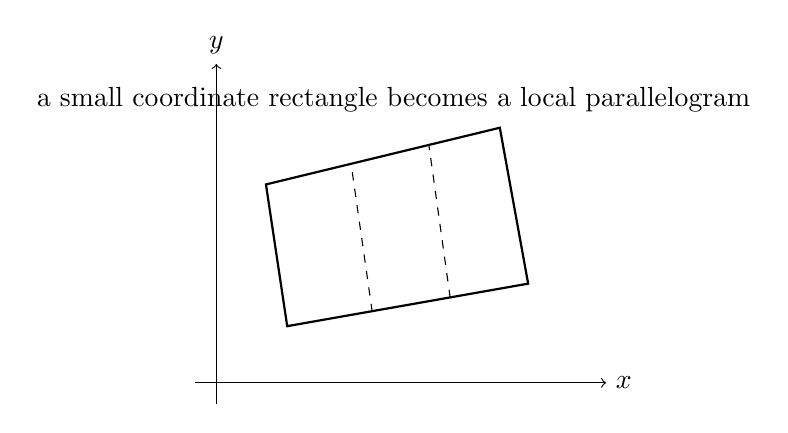
\begin{tikzpicture}[scale=0.9]
\draw[->] (-0.3,0)--(5.5,0) node[right]{$x$};
\draw[->] (0,-0.3)--(0,4.5) node[above]{$y$};
\draw[thick] (1.0,0.8) -- (4.4,1.4) -- (4.0,3.6) -- (0.7,2.8) -- cycle;
\draw[dashed] (2.2,1.0)--(1.9,3.1);
\draw[dashed] (3.3,1.2)--(3.0,3.35);
\node at (2.5,4.0) {a small coordinate rectangle becomes a local parallelogram};
\end{tikzpicture}
\caption{The Jacobian maps infinitesimal coordinate cells into locally distorted cells. Its determinant gives the signed area or volume scale factor.}
\label{fig:jacobian-deformation}
\end{figure}

\subsection{The Hessian Matrix}

For a twice differentiable scalar function $f:\mathbb R^n\to\mathbb R$, the Hessian is

\begin{equation}
\boxed{
H_f
=
\begin{pmatrix}
\dfrac{\partial^2f}{\partial x_1^2} & \cdots & \dfrac{\partial^2f}{\partial x_1\partial x_n}\\[6pt]
\vdots & \ddots & \vdots\\[6pt]
\dfrac{\partial^2f}{\partial x_n\partial x_1} & \cdots & \dfrac{\partial^2f}{\partial x_n^2}
\end{pmatrix}.
}
\label{eq:hessian}
\end{equation}

When mixed partials are continuous, the Hessian is symmetric. Its eigenvectors identify principal curvature directions, and its eigenvalues measure the corresponding second-order curvature.

For two variables,

\[
H_f
=
\begin{pmatrix}
f_{xx} & f_{xy}\\
f_{yx} & f_{yy}
\end{pmatrix}.
\]

\subsection{Local Extrema and the Second-Derivative Test}

A critical point satisfies

\[
f_x(a,b)=0,
\qquad
f_y(a,b)=0.
\]

Define

\[
D=f_{xx}f_{yy}-f_{xy}^2.
\]

At a critical point:

\begin{itemize}
\item if $D>0$ and $f_{xx}>0$, $f$ has a local minimum;
\item if $D>0$ and $f_{xx}<0$, $f$ has a local maximum;
\item if $D<0$, the point is a saddle point;
\item if $D=0$, the test is inconclusive.
\end{itemize}

Equivalently, in terms of Hessian eigenvalues:

\begin{itemize}
\item all positive eigenvalues imply a local minimum;
\item all negative eigenvalues imply a local maximum;
\item mixed signs imply a saddle point.
\end{itemize}

\begin{bookexample}[Minimum and Saddle]
For
\[
f(x,y)=x^2+4y^2,
\]
the only critical point is $(0,0)$ and
\[
H_f=
\begin{pmatrix}
2&0\\0&8
\end{pmatrix}.
\]
Both eigenvalues are positive, so the origin is a strict local minimum.

For
\[
g(x,y)=x^2-y^2,
\]
\[
H_g=
\begin{pmatrix}
2&0\\0&-2
\end{pmatrix},
\]
whose eigenvalues have opposite signs. The origin is therefore a saddle point.
\end{bookexample}

\begin{figure}[htbp]
\centering
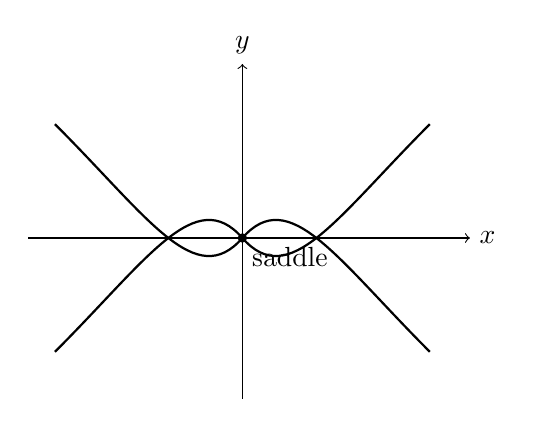
\begin{tikzpicture}[scale=0.85]
\draw[->] (-3.2,0)--(3.4,0) node[right]{$x$};
\draw[->] (0,-2.4)--(0,2.6) node[above]{$y$};
\draw[thick] (-2.8,-1.7) .. controls (-1.4,-0.3) and (-0.7,0.8) .. (0,0)
.. controls (0.7,-0.8) and (1.4,0.3) .. (2.8,1.7);
\draw[thick] (-2.8,1.7) .. controls (-1.4,0.3) and (-0.7,-0.8) .. (0,0)
.. controls (0.7,0.8) and (1.4,-0.3) .. (2.8,-1.7);
\fill (0,0) circle (2pt) node[below right]{saddle};
\end{tikzpicture}
\caption{At a saddle point the function curves upward in one principal direction and downward in another.}
\label{fig:hessian-saddle}
\end{figure}

\subsection{Applications in Thermodynamics}

Thermodynamic variables are often connected by state functions such as

\[
U=U(S,V,N),
\]

where $U$ is internal energy, $S$ entropy, $V$ volume, and $N$ particle number. Its differential is

\begin{equation}
\boxed{
dU
=
\left(\frac{\partial U}{\partial S}\right)_{V,N}dS
+
\left(\frac{\partial U}{\partial V}\right)_{S,N}dV
+
\left(\frac{\partial U}{\partial N}\right)_{S,V}dN.
}
\end{equation}

Thermodynamics identifies

\[
T=\left(\frac{\partial U}{\partial S}\right)_{V,N},
\qquad
-p=\left(\frac{\partial U}{\partial V}\right)_{S,N},
\qquad
\mu=\left(\frac{\partial U}{\partial N}\right)_{S,V}.
\]

Thus

\[
\boxed{dU=T\,dS-p\,dV+\mu\,dN.}
\]

The subscripts are essential: a thermodynamic partial derivative is defined by specifying which variables remain fixed.

\subsection{Applications in Electromagnetism}

An electrostatic potential $V(x,y,z)$ determines the electric field through

\[
\mathbf E=-\nabla V.
\]

Its Cartesian components are

\[
E_x=-\frac{\partial V}{\partial x},
\qquad
E_y=-\frac{\partial V}{\partial y},
\qquad
E_z=-\frac{\partial V}{\partial z}.
\]

The potential also satisfies Poisson's equation,

\[
\frac{\partial^2V}{\partial x^2}
+
\frac{\partial^2V}{\partial y^2}
+
\frac{\partial^2V}{\partial z^2}
=-\frac{\rho}{\varepsilon_0},
\]

or Laplace's equation when $\rho=0$.

\subsection{Applications in Fluid Mechanics}

A fluid velocity field is

\[
\mathbf v(x,y,z,t)
=
(v_x,v_y,v_z).
\]

The rate of change of a scalar quantity $f$ experienced by a moving fluid element is

\begin{equation}
\boxed{
\frac{Df}{Dt}
=
\frac{\partial f}{\partial t}
+
\mathbf v\cdot\nabla f.
}
\label{eq:material-derivative}
\end{equation}

This material derivative combines local time variation and advection through space. It is one of the central operators of continuum mechanics.

\subsection{Applications in Quantum Mechanics}

The non-relativistic wavefunction

\[
\psi(x,y,z,t)
\]

is a complex field over space and time. The time-dependent Schr\"odinger equation is

\begin{equation}
\boxed{
i\hbar\frac{\partial\psi}{\partial t}
=
\left[
-\frac{\hbar^2}{2m}
\left(
\frac{\partial^2}{\partial x^2}
+
\frac{\partial^2}{\partial y^2}
+
\frac{\partial^2}{\partial z^2}
\right)
+V(x,y,z,t)
\right]\psi.
}
\label{eq:schrodinger-partial-derivatives}
\end{equation}

The first partial derivative in time controls evolution, while the second spatial partial derivatives represent kinetic energy through the Laplacian.

\begin{bookexample}[Separable Wavefunction]
If
\[
\psi(x,t)=X(x)T(t),
\]
then
\[
\frac{\partial\psi}{\partial t}=X(x)\frac{dT}{dt},
\qquad
\frac{\partial^2\psi}{\partial x^2}=T(t)\frac{d^2X}{dx^2}.
\]
Partial differentiation allows one factor to be treated as constant while differentiating the other, enabling separation of variables.
\end{bookexample}

\subsection{Common Mistakes}

\begin{bookwarning}[Frequent Errors]
\begin{itemize}
\item Forgetting which variables are held fixed.
\item Confusing $\partial f/\partial t$ with the total derivative $df/dt$.
\item Assuming that existing partial derivatives automatically imply differentiability.
\item Omitting the Jacobian determinant in a change of integration variables.
\item Applying the Hessian test at a point that is not critical.
\item Treating $\nabla$ as an ordinary numerical vector before it acts on a field.
\end{itemize}
\end{bookwarning}

\subsection{Exercises}

\begin{enumerate}
\item Use the limit definition to calculate $f_x$ and $f_y$ for $f(x,y)=xy^2+x^2$.
\item Find the tangent plane to $z=e^{xy}$ at $(1,0)$.
\item Estimate the change in $f(x,y)=\sqrt{x^2+y^2}$ when $(x,y)$ changes from $(3,4)$ to $(3.02,3.99)$.
\item Compute the directional derivative of $f(x,y)=x^2-y^2$ at $(2,1)$ in the direction from $(2,1)$ to $(5,5)$.
\item Find the Jacobian determinant of the transformation $u=x+y$, $v=x-y$.
\item Derive the polar area element $dx\,dy=r\,dr\,d\theta$.
\item Classify the critical points of $f(x,y)=x^3-3x+y^2$.
\item For $T(x,y,t)=e^{-t}(x^2+y^2)$ and a path $x=\cos t$, $y=\sin t$, compute $dT/dt$.
\item Show that the Hessian of $f(x,y)=\ln(x^2+y^2)$ is symmetric away from the origin.
\item For a wavefunction $\psi(x,t)=Ae^{-\alpha x^2}e^{-i\omega t}$, compute $\partial\psi/\partial t$ and $\partial^2\psi/\partial x^2$.
\end{enumerate}

\subsection*{Summary}

Partial derivatives extend ordinary differentiation to functions of many variables. Each coordinate partial derivative is defined by an ordinary one-dimensional limit along a coordinate slice. When the function is differentiable, these partial derivatives combine into the best local linear approximation, the tangent plane, and the total differential.

Directional derivatives describe change in arbitrary directions. Jacobian matrices represent the first-order linearization of vector-valued mappings, while Jacobian determinants measure local changes of area and volume under coordinate transformations. Hessian matrices collect second derivatives and reveal curvature, stability, and the character of critical points.

In physics, these ideas appear in thermodynamic state relations, electric and gravitational potentials, fluid flow, continuum mechanics, and quantum wave equations. The next section develops the gradient, which packages the coordinate partial derivatives of a scalar field into a single geometric vector pointing in the direction of maximum increase.
